% Figure source. `npm run notes -- build stat497` compiles it to the PDF the
% notes include and to time-order.svg for the web page. The same five values
% in two orders. The handwritten legend lists Y as 3, 4, 1, 5, 6; the plot and
% the point of the figure (each value once) make it 3, 4, 1, 5, 2.
\documentclass[tikz,border=4pt]{standalone}
\usepackage{libertinus}
\usepackage{libertinust1math}
\usepackage{pgfplots}
\pgfplotsset{compat=1.18}
\definecolor{accent}{HTML}{1D4E89}
\definecolor{caution}{HTML}{9B2C2C}
\definecolor{quiet}{HTML}{6B7280}
\definecolor{hair}{HTML}{D5D9DF}

\begin{document}
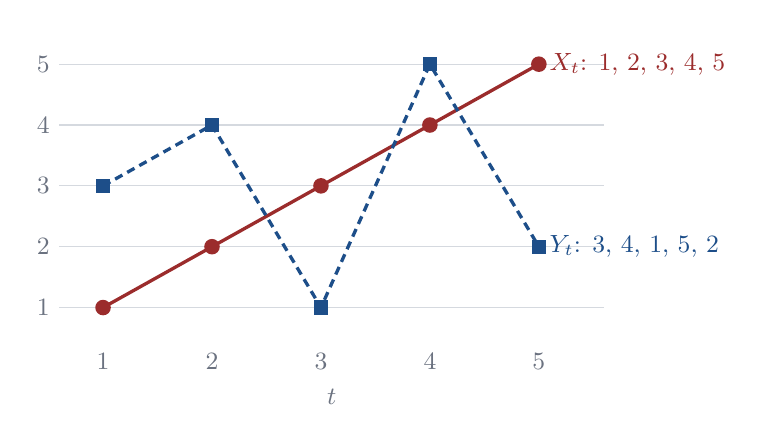
\begin{tikzpicture}
  \begin{axis}[
      width=8.5cm, height=5.6cm,
      xmin=0.6, xmax=5.6, ymin=0.4, ymax=5.6,
      xtick={1,...,5}, ytick={1,...,5},
      xlabel={$t$}, xlabel style={font=\small, text=quiet},
      axis line style={draw=none}, tick style={draw=none},
      ymajorgrids, grid style={hair, line width=.4pt},
      tick label style={font=\small, text=quiet},
      clip=false,
    ]
    \addplot[caution, line width=1.2pt, mark=*, mark size=2.2pt]
      coordinates {(1,1) (2,2) (3,3) (4,4) (5,5)}
      node[right, font=\small, text=caution] {$X_t$: 1, 2, 3, 4, 5};
    \addplot[accent, densely dashed, line width=1.2pt, mark=square*, mark size=2pt,
      mark options={solid}] coordinates {(1,3) (2,4) (3,1) (4,5) (5,2)}
      node[right, font=\small, text=accent] {$Y_t$: 3, 4, 1, 5, 2};
  \end{axis}
\end{tikzpicture}
\end{document}
